% !TeX spellcheck = en_US
% !TeX encoding = UTF-8

% COMPILE WITH:
% `latexmk`
% You need lualatex and biber (in all TeXLive distributions)

\documentclass[
    numbers=noenddot,
    %listof=totoc,
    parskip=half-,
    fontsize=12pt,
    paper=a4,
    oneside,
    titlepage,
    bibliography=totoc,
    chapterprefix=false,
    headheight=30pt,
    footheight=30pt
%    draft
]{scrbook}

\setcounter{secnumdepth}{3}

% use lualatex or xelatex
\usepackage{fontspec}
\usepackage{graphicx}
\usepackage[onehalfspacing]{setspace}
\usepackage{setspace}
% better language support
\usepackage{polyglossia}
\setdefaultlanguage{english}
\setotherlanguage{german}

\usepackage{tocbasic}
\usepackage{booktabs}
\usepackage{multicol}
\usepackage{multirow}
\usepackage{rotating} % 用于旋转表格
\usepackage{siunitx}

\usepackage{tikz}
\usepackage{amsmath}
\renewcommand{\vec}{\mathbf}

\usepackage[]{scrlayer-scrpage}

% better bibliography (biblatex style)
% use biber to compile
\usepackage[citestyle=alphabetic, bibstyle=alphabetic, sorting=nyt, backend=biber, language=english, backref=true, maxcitenames=2]{biblatex}

% better quotes
% use \enquote{text}
\usepackage[autostyle,english=american,german=quotes]{csquotes}
\addbibresource{bibliography.bib}

% appendix
\usepackage[titletoc]{appendix}

% where to put all images and figures
\graphicspath{{images/}}

% YOUR PACKAGES
\usepackage{hyperref}
\usepackage{amssymb}
\usepackage{float}
\usepackage{subfig}


% Title
\title{TITLE}

% Author
\author{AUTHOR}

% Date
\date{\today}

% CHOOSE ACCORDINGLY
\newcommand{\thesisType}{Bachelorarbeit}
% \newcommand{\thesisType}{Masterarbeit}

\makeatletter
\let\thetitle\@title
\let\theauthor\@author
\let\thedate\@date
\makeatother

\pagestyle{scrheadings}

\begin{document}

%%%%%%%%%%%%%%%%%%%%%%%%%%%%%%%%%%%%%%%%%%%%%%%%%%%%%%%%%%%%%%%%%%%%%%%%%%%%%%%%%%%%%%%%%
\frontmatter
% CHOOSE ACCORDINGLY
% !TeX spellcheck = en_US
% !TeX encoding = UTF-8
\begin{titlepage}
    \centering
    \begin{onehalfspace}
    	\begin{german}
        	% \includegraphics[width=7cm]{uni-logo.png}\\
        	\vspace{1.0cm}
        	\large {\bfseries Chair of Computer Science 6 (i6)\\Learning on Graphs (LoG)} \\

        	\vspace{2.5cm}

            \begin{doublespace}
            	\textenglish{\textsf{\Huge{Exploration of the Influence of Graph Parameters on the Generalization Error of Graph Neural Networks}}}
            \end{doublespace}

        	\vspace{2cm}

            \Large{Bachelor Thesis from}\\

        	\vspace{1cm}

        	{\bfseries \large{Wensheng Zhang}}

        	\vfill

        	{\large
        		\begin{tabular}[l]{cc}
                        \textsc{Supervisor}\\
        			Chendi Qian, M.~Sc. \\
        			\textsc{1.Examiner}\\
        			Prof.~Dr.~Christopher Morris \\
                        \textsc{2.Examiner}\\
        			Prof.~Michael Schaub
        		\end{tabular}
        	}

        	\vspace{1.5cm}

        	\parbox{\linewidth}{\hrule\strut}

            \vfill

	    \textgerman{\thedate}
    	\end{german}
    \end{onehalfspace}
\end{titlepage}

% % !TeX spellcheck = en_US
% !TeX encoding = UTF-8
\begin{titlepage}
    \centering
    \begin{onehalfspace}
    	\begin{german}
        	\includegraphics[width=7cm]{uni-logo.png}\\
        	\vspace{1.0cm}
        	\large {\bfseries Lehrstuhl für Informatik mit Schwerpunkt\\ \textenglish{Digital Libraries and Web Information Systems}} \\

        	\vspace{2.5cm}

            \begin{doublespace}
            	\textenglish{\textsf{\Huge{\thetitle}}}
            \end{doublespace}

        	\vspace{2cm}

            \Large{Masterarbeit von}\\

        	\vspace{1cm}

        	{\bfseries \large{\theauthor}}

        	\vfill

        	{\large
        		\begin{tabular}[l]{cc}
        			\textsc{1.~Prüfer} & \textsc{2.~Prüfer} \\
        			Prof.~Dr.~Siegfried Handschuh & <ZWEITER PRÜFER>
        		\end{tabular}
        	}

        	\vspace{1.5cm}

        	\parbox{\linewidth}{\hrule\strut}

            \vfill

	    \textgerman{\thedate}
    	\end{german}
    \end{onehalfspace}
\end{titlepage}


\addtocontents{toc}{\setcounter{tocdepth}{3}} 
\tableofcontents
\newpage

% -- Acknowledgements (optional)
% % !TeX spellcheck = en_US
% !TeX encoding = UTF-8
\chapter*{Acknowledgments}
First of all, I would like to thank Prof. Michael Schaub and Prof. Volkmar Schulz for their great support for my thesis. 
Secondly I would like to thank my superadvisor Franziska Schrank for giving me the opportunity to do this thesis, 
and also for her help in understanding the content of the thesis at the beginning and for her help in the content and code throughout my entire bachelor thesis time.

% \cleardoublepage
% \addcontentsline{toc}{chapter}{Acknowledgements}
% \newpage
\cleardoublepage
\phantomsection
\addcontentsline{toc}{chapter}{Acknowledgements}
\chapter*{Acknowledgements}
First, I would like to thank Prof.~Christopher Morris and Prof.~Michael Schaub for giving me the opportunity of this thesis. 
Secondly, I would like to thank my supervisor Chendi Qian for the great support to do this thesis, and also for his help in understanding the content of the thesis at the beginning, and for his help in the content and code throughout my entire bachelor thesis time.


% -- List of figures
\thispagestyle{empty}
\cleardoublepage
\phantomsection
\addcontentsline{toc}{chapter}{List of figures}
\listoffigures
\newpage

% -- List of tables
\thispagestyle{empty}
\cleardoublepage
\phantomsection
\addcontentsline{toc}{chapter}{List of tables}
\listoftables
\newpage


% -- ABSTRACT
\cleardoublepage
\phantomsection
% !TeX spellcheck = en_US
% !TeX encoding = UTF-8
\chapter*{Abstract}
The goal of this bachelor thesis is to understand empirically how graph parameters/characteristics influence the generalization error of Graph Neural Networks (GNNs).
% -- ABSTRACT
% \cleardoublepage
% \phantomsection
% % !TeX spellcheck = en_US
% !TeX encoding = UTF-8
\chapter*{Abstract}
The goal of this bachelor thesis is to understand empirically how graph parameters/characteristics influence the generalization error of Graph Neural Networks (GNNs).




%%%%%%%%%%%%%%%%%%%%%%%%%%%%%%%%%%%%%%%%%%%%%%%%%%%%%%%%%%%%%%%%%%%%%%%%%%%%%%%%%%%%%%%%%
\mainmatter

% -- Chapters
% following IMRaD structure
% adjust for your liking
\chapter{Introduction}\label{chap:introduction}
Graph representation learning has emerged as a prominent area within machine learning, driven by its capacity to model relationships in graph-structured data effectively. Graph Neural Networks (GNNs)~\cite{gori2005new}, also known as deep learning on graphs, are a class of neural networks that can operate on graph-structured data, such as social networks~\cite{easley2010networks}, biological networks~\cite{barabasi2004network}, and images~\cite{simonovsky2017dynamic}. GNNs use the structure of a graph to perform ``message passing'', allowing information to propagate across nodes and edges. The key idea is to iteratively aggregate and update node features by exchanging information with local neighboring nodes, which allows GNNs to capture the structural information of the graph. This information is then used to make predictions. GNNs have been demonstrated to be effective in a wide range of tasks, such as node classification~\cite{hamilton2017inductive}, edge prediction~\cite{kipf2016variational}, and graph classification~\cite{gilmer2017neural}. Popular GNNs in recent years include Graph Convolutional Network (GCN)~\cite{kipf2016semi}, Graph Attention Network (GAT)~\cite{velickovic2020pointer}, and Message Passing Neural Network (MPNN)~\cite{gilmer2017neural}.  

From the perspective of \cite{morris2024futuredirectionstheorygraph}, the behavior of GNNs remains insufficiently understood, particularly with respect to how graph parameters/characteristics influence their empirical generalization error. This thesis aims to address this gap by conducting an empirical investigation into the impact of graph parameters on the generalization performance of GNNs.

To achieve this objective, two sets of experiments were conducted:

First, graph parameters were computed for a set of 49 datasets selected from the TUDataset~\cite{morris2020tudataset} In graph theory, each graph have its own unique properties, such as the average degree. In graph theory, graph parameters are used to quantify them. A dataset consist of multiple graphs, each with its graph parameter. For each dataset, the average values of the specified graph parameters were calculated across all graphs. In this thesis, 49 datasets from the TUDataset~\cite{morris2020tudataset} were used for the calculation.

Secondly, various GNN architectures were trained across multiple datasets, and it is revealed that their generalization abilities varied. The analysis identified a notable correlation between generalization capabilities and specific graph-theoretic parameters.

The thesis is organized as follows:
Chapter~\ref{chap:background} provides background information on graph neural networks and generalization. Chapter~\ref{chap:experiments} describes the methodology used to conduct the experiments. Chapter~\ref{chap:results} presents the experimental results and discusses the results and their implications. Finally, Chapter~\ref{chap:conclusions} concludes the thesis and discusses future work.

\section{Related work}
The subsequent section examines related work on GNNs and a focus on their generalization capabilities.

\subsection{Graph Neural Networks}
GNNs were initially proposed by Gori et al.~\cite{gori2005new} and Scarselli et al.~\cite{scarselli2008graph} as a variant of recurrent neural networks. These models demonstrated its significant generalization capabilities, marking a foundational step in the development of graph-based learning frameworks. The work of Kipf and Welling~\cite{kipf2016semi} introduced the Graph Convolutional Networks (GCN) model, which received widespread attention from the research community. Gilmer et al.~\cite{gilmer2017neural} introduced the Message Passing Neural Networks (MPNN) model, which demonstrated the significant results on the molecular property prediction benchmark. Velickovic et al.~\cite{velivckovic2017graph} proposed the Graph Attention Networks (GAT) model, which uses attention mechanisms to aggregate information from neighboring nodes. Brody et al.~\cite{brody2021attentive} proposed the GATv2 model, which outperforms the GAT model by introducing a dynamic graph attention variant.

\subsection{Generalization}
While significant progress has been made in understanding the generalization properties of Feed-forward Neural Networks (FNNs) and Recurrent Neural Networks (RNNs). The generalization capabilities of GNNs remain underexplored, primarily due to the challenges posed by the irregular and non-Euclidean nature of graph structures.

Golowich et al.~\cite{golowich2018size} showed the generalization abilities of FNNs with Rademacher complexity. The work of Zhang et al.~\cite{zhang2018stabilizing} used SVD-based parameterization to improve the generalization by effectively addressing gradient issues.

In terms of RNNs, Chen et al.~\cite{chen2019generalization} studied the generalization properties of vanilla RNNs as well as their variants. Z. Allen-Zhu et al.~\cite{allen2019can} demonstrates that vanilla SGD enables RNNs to efficiently learn concept classes and overcomes prior exponential generalization bounds. 

In contrast to the FNNs and RNNs, GNNs deal with irregular data structures. The related work on the generalization of GNNs is limited. Scarselli et al.~\cite{scarselli2018vapnik} explored the generalization ability of GNNs by using the Vapnik-Chervonenkis (VC) dimension and further indicated that the generalization ability of such models improve as the number of connected nodes. After that, Garg et al.~\cite{garg2020generalization} studied the generalization ability of GNNs via Rademacher bounds. In comparison to the work of Scarselli et al., Garg et al. provided a tighter bound on the generalization error of GNNs.

Nevertheless, Morris et al.~\cite{morris2024futuredirectionstheorygraph} pointed out that the generalization ability of GNNs is still not well understood. The bounds established in these studies typically rely solely on general graph parameters, such as the maximum degree or total number of nodes, while often overlooking more expressive graph parameters.
\chapter{Background}\label{chap:background}
The following sections provide an overview of the concepts and methods related to graph theory, machine learning, and graph neural networks. 

\section{Notation}
First, it is necessary to define key terms related to graphs. In graph theory, it is assumed that $\mathcal{G}=(\mathcal{V},\mathcal{E})$ is an undirected graph, where $\mathcal{V}$ is the set of nodes and $\mathcal{E}  \subseteq \{\{v,w\}\mid v,w \in \mathcal{V} , v \neq w\}$ is the set of edges. The term $\mathbb{G}$ is used to represent the set of all possible graphs. The neighborhood of a node $v$ is denoted as $N(v)$, defined as $N(v) = \{w \mid \{v,w\} \in \mathcal{E}\}$. The degree of a node $v$, denoted as $d(v)$, is the number of neighbors of $v$, that is, $d(v) = |N(v)|$. 

The adjacency matrix $\vec{A} \in \{0,1\}^{|\mathcal{V}| \times |\mathcal{V}|}$ is a matrix that represents the connections between nodes in the graph. The element $a_{ij}$ of the adjacency matrix is 1 if there is an edge between node $v_i$ and node $v_j$, and 0 otherwise.

In addition to the nodes and edges that comprise the graph, it is possible to attach a more complex set of data to each node. A feature vector $\vec{x}_n\in \mathbb{R}^D$ with $0 \leq n < |\mathcal{V}|$, is attached to a node $v_n$, and in some cases, edge feature vectors are also included, where $D$ is the number of dimension of feature vectors. Then a matrix $\vec{X} \in \mathbb{R}^{|\mathcal{V}|\times D}$ can be constituted by stacking thesis node features vectors:

$$
    \vec{X} = \begin{bmatrix}
    \vec{x}_1 \\
    \vec{x}_2 \\
    \vdots \\
    \vec{x}_{|V|}
    \end{bmatrix}
$$

These vectors can be used to characterize graphs or nodes in graphs.

\section{Machine learning}
In the subsequent section, an overview of the concepts and methodologies associated with machine learning is presented. 

\paragraph{Supervised learning}
Machine learning can be roughly divided into three categories: supervised learning, unsupervised learning, and reinforcement learning~\cite{bishop2006pattern}.

Supervised learning is a type of machine learning that involves training a model on a labeled dataset. The model is trained to learn the relationship between the input features and the output labels. The goal is to learn a mapping from the input features to the output labels so that the model can make predictions on new, unseen data. One common task in supervised learning is classification, where the goal is to assign each input vector to one of a finite number of classes (categories). In the graph learning context, the predicted output can be a label for each node in the graph, a label for the entire graph, or a label for each edge in the graph, e.g. node classification, graph classification, and link prediction~\cite{velivckovic2023everything}.

\paragraph{Feed-forward Neural Networks}

Feed-forward Neural Networks (FNNs), also known as multilayer perceptrons (MLPs), are a type of neural network that consists of multiple layers of neurons. The neurons in each layer are connected to the neurons in the next layer, and the output of each neuron is computed as a weighted sum of the inputs followed by a non-linear activation function. The output of the network is computed by passing the input through the network and computing the output of the final layer. The weights of the network are learned by using an optimization algorithm such as gradient descent. Feed-forward neural networks are a powerful tool for learning complex patterns in data and have been successfully applied to a wide range of tasks, such as image recognition, speech recognition, and natural language processing.

The function of a feed-forward neural network can be written as

$$ 
    \vec{y} = f(\vec{W}^{(L)} \cdot f(\vec{W}^{(L-1)} \cdot \ldots \cdot f(\vec{W}^{(1)} \cdot \vec{x} + \vec{b}^{(1)}) + \vec{b}^{(2)}) + \ldots + \vec{b}^{(L)})
$$

where $\vec{x}\in \mathbb{R}^D$ is the input vector, $\vec{W}^{(i)}$ and $\vec{b}^{(i)}$ are the weights and biases of the $i$-th layer, and $f$ is the activation function. The output $\vec{y}$ is the predicted output of the network. $L$ is denoted as the depth of the network. See Figure~\ref{fig:neural_network} for an illustration of a single neuron in a feed-forward neural network.

\usetikzlibrary{decorations.pathreplacing}
\begin{figure}[h!]
    \centering
\begin{tikzpicture}[>=stealth, scale=1.5, every node/.style={scale=1.2}]

    % Input signals
    \node at (-1.5, 1.5) (x1) {$x_1$};
    \node at (-1.5, 0.5) (x2) {$x_2$};
    \node at (-1.5, -1) (xm) {$x_m$};
    \node at (-1.5, -0.25) (dots) {$\vdots$};
    
    % Input brackets
    \draw[decorate, decoration={brace, amplitude=5pt}] (-1.8, -1.1) -- (-1.8, 1.6) node[midway, left, xshift=-0.2cm, scale=0.8] {Input vector};
        
    % Weights
    \node[draw, circle] at (0.3, 1.5) (w1) {$w_1$};
    \node[draw, circle] at (0.3, 0.5) (w2) {$w_2$};
    \node[draw, circle] at (0.3, -1) (wm) {$w_m$};
    
    \draw[->] (x1) -- (w1);
    \draw[->] (x2) -- (w2);
    \draw[->] (xm) -- (wm);

    % Sum node
    \node[draw, circle] at (2, 0) (sum) {$\Sigma$};
    
    % Weighted connections to sum
    \draw[->] (w1) -- (sum);
    \draw[->] (w2) -- (sum);
    \draw[->] (wm) -- (sum);
    
    % Bias
    \node[scale=0.8] at (2, 1.6) (biasText) {Bias};
    \node at (2, 1.2) (biasEq) {$b$};
    \draw[->] (biasEq) -- (sum);
    
    % Activation function
    \node[draw, rectangle] at (3.5, 0) (activation) {$\phi(\cdot)$};
    \node at (5, 0) (y) {$y$};
    \draw[->] (sum) -- (activation);
    \draw[->] (activation) -- (y);
    
    % Activation function label
    \node[scale=0.8] at (3.5, 0.6) {Activation function};
    
    % Weight label
    \node[scale=0.8] at (0.3, -1.7) {Weights};
    
    % Sum label
    \node[scale=0.8] at (2.05, -0.5) {Sum};
\end{tikzpicture}
\caption{The diagram illustrates the basic structure of a neuron in an artificial neural network. Inputs $x_1, x_2, \ldots, x_m \in \mathbb{R}$ are multiplied by their respective weights $w_1, w_2, \ldots, w_m \in \mathbb{R}$ and summed together including a bias term $b$. The result is then passed through an activation function $\phi(\cdot)$ to produce the output $y$.}
\label{fig:neural_network}
\end{figure}

\paragraph{Loss function}
The loss function is a function that measures the difference between the predicted output of a model and the true output. The goal of training a machine learning model is to minimize the loss function, which is done by adjusting the parameters of the model using an optimization algorithm such as gradient descent. The choice of loss function depends on the task at hand. For classification tasks, the cross-entropy loss function is commonly used, while for regression tasks, the mean squared error loss function is often used.

The cross-entropy loss function is defined as 

$$
    L(\vec{y}, \hat{\vec{y}}) = -\sum_{i} \vec{y_i} \log(\hat{\vec{y}}_i)
$$

where $\vec{y}$ is the true output, $\hat{\vec{y}}$ is the predicted output, and $i$ is the index of the classes. The cross-entropy loss function is used to measure the difference between the true output and the predicted output of a classification model. See Figure~\ref{fig:loss_function} for a simple example of a cost function surface in machine learning.

\begin{figure}[H]
    \centering
    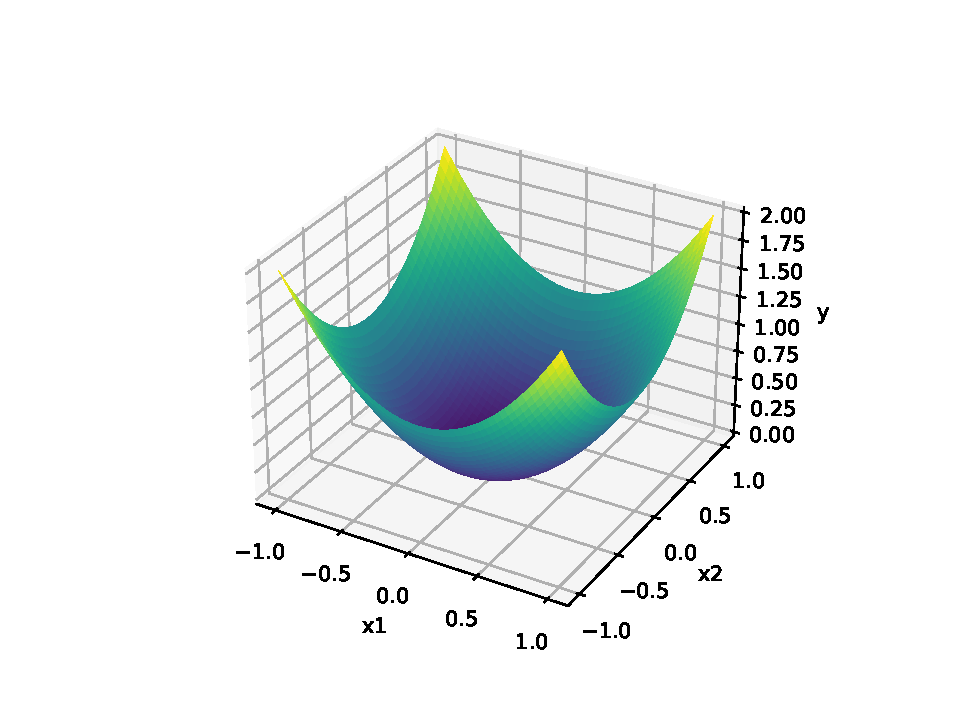
\includegraphics[width=0.8\textwidth]{loss_function.pdf}
    \caption{A 3D representation of a cost function surface used in machine learning optimization. The x1 and x2 axes represent input parameters, while the y-axis represents the cost value. The surface highlights the nature of the optimization landscape.}
    \label{fig:loss_function}
\end{figure}

\paragraph{Activation function}
An activation function is a non-linear function that is applied to the output of a neuron in a neural network. The activation function introduces non-linearity into the network, allowing it to learn complex patterns in the data. There are many activation functions that can be used in neural networks, such as the Sigmoid function, the Hyperbolic Tangent (Tanh) function, the Rectified Linear Unit (ReLU) function \cite{nair2010rectified} and its variant Leaky Rectified Linear Unit (LeakyReLU) \cite{xu2015empirical}. The ReLU function is one of the most commonly used activation functions in deep learning because it is simple and computationally efficient. The ReLU function is defined as:

\begin{equation*}
    \textrm{ReLU}(x)=\max(0,x)
\end{equation*}

And its variant, the LeakyReLU function, is defined as:

\begin{equation*}
    \mathrm{LeakyReLU}(x) = 
    \begin{cases} 
        x, & \text{if } x > 0 \\
        \alpha x, & \text{otherwise}
    \end{cases}
\end{equation*}

where $\alpha$ is a small positive constant that controls the slope of the function for negative values of $x$.

The ReLU function is used to introduce non-linearity into the network and has been shown to be effective in training deep neural networks.


\paragraph{Gradient descent}
Gradient descent is an optimization algorithm used to minimize a function by iteratively moving in the direction of the steepest decrease of the function. The algorithm works by computing the gradient of the function at a given point and then updating the point in the direction of the negative gradient. The update rule is given by

\begin{equation} \label{eq:gradient_descent}
    \vec{W}^{(t+1)} = \vec{W}^{(t)} - \alpha \nabla f(\vec{W}^{(t)})
\end{equation}

where $\vec{W}^{(t)}$ is the parameter vector at iteration $t$, $\alpha$ is the learning rate, and $\nabla f(\vec{W}^{(t)})$ is the gradient of the function $f$ with respect to the parameters $\vec{W}^{(t)}$. The learning rate $\alpha$ is a hyperparameter that controls the step size of the update. Gradient descent is a popular optimization algorithm used in machine learning to train neural networks and other models.

\paragraph{Stochastic gradient descent}
Stochastic gradient descent~\cite{robbins1951stochastic} is a variant of gradient descent that uses a random sample of the training data to compute the gradient at each iteration. The algorithm works by randomly selecting a mini-batch of data points from the training dataset, computing the gradient of the loss function with respect to the mini-batch, and then updating the parameters based on the gradient. The update rule is given by

\begin{equation} \label{eq:stochastic_gradient_descent}
    \vec{W}^{(t+1)} = \vec{W}^{(t)} - \alpha \nabla f(\vec{W}^{(t)}, \vec{x}^{(t)})
\end{equation}

where $\vec{W}^{(t)}$ is the parameter vector at iteration $t$, $\alpha$ is the learning rate, $\nabla f(\vec{W}^{(t)}, \vec{x}^{(t)})$ is the gradient of the function $f$ with respect to the parameters $\vec{W}^{(t)}$ and the mini-batch $\vec{x}^{(t)}$. Stochastic gradient descent is more computationally efficient than standard gradient descent~\ref{eq:gradient_descent} and can be used to train large-scale machine learning models.

\paragraph{Optimization algorithm}
An optimization algorithm is an algorithm used to minimize a function by iteratively updating the parameters of the model. The goal is to find the set of parameters that minimizes the loss function. Gradient descent is a common optimization algorithm used in machine learning, but there are many variants of gradient descent that are designed to improve convergence speed and stability. Some popular optimization algorithms include Adam~\cite{kingma2014adam}, RMSprop~\cite{graves2013generating}, and Adagrad~\cite{duchi2011adaptive}. These algorithms use different strategies to update the parameters of the model and can be more effective than standard gradient descent in certain situations. 

\paragraph{Early stopping}
Early stopping \cite{morgan1989generalization}\cite{prechelt2002early} is a technique used to prevent overfitting in machine learning models. The idea is to monitor the performance of the model on a validation dataset during training and stop training when the performance starts to degrade. This is done by keeping track of the validation loss and stopping training when the validation loss stops decreasing or starts to increase. Early stopping is used to prevent the model from memorizing the training data and to obtain a more generalizable model. 

\paragraph{Cross-validation}
Cross-validation is a technique used to evaluate the performance of a machine learning model. The idea is to split the dataset into multiple subsets, or folds, and train the model on one subset while evaluating it on the remaining subsets. This process is repeated multiple times, with each subset used as the test set once. The performance of the model is then averaged over all the folds to obtain an estimate of the model's generalization performance. Cross-validation is used to prevent overfitting and to obtain a more accurate estimate of the model's performance. See Figure~\ref{fig:cross-validation} for an example of 5-fold cross-validation.


\begin{center}
    \begin{tikzpicture}[scale=1.2]

    % Run 1
    \draw[thick] (0, 5) rectangle (5, 5.5);
    \fill[red!70] (0, 5) rectangle (1, 5.5);
    \draw[thick] (1, 5) -- (1, 5.5);
    \draw[thick] (2, 5) -- (2, 5.5);
    \draw[thick] (3, 5) -- (3, 5.5);
    \draw[thick] (4, 5) -- (4, 5.5);

    \node[right=6pt] at (5, 5.25) {run 1};

    % Run 2
    \draw[thick] (0, 4.5) rectangle (5, 5);
    \fill[red!70] (1, 4.5) rectangle (2, 5);
    \draw[thick] (1, 4.5) -- (1, 5);
    \draw[thick] (2, 4.5) -- (2, 5);
    \draw[thick] (3, 4.5) -- (3, 5);
    \draw[thick] (4, 4.5) -- (4, 5);

    \node[right=6pt] at (5, 4.75) {run 2};

    % Run 3
    \draw[thick] (0, 4) rectangle (5, 4.5);
    \fill[red!70] (2, 4) rectangle (3, 4.5);
    \draw[thick] (1, 4) -- (1, 4.5);
    \draw[thick] (2, 4) -- (2, 4.5);
    \draw[thick] (3, 4) -- (3, 4.5);
    \draw[thick] (4, 4) -- (4, 4.5);
    \node[right=6pt] at (5, 4.25) {run 3};

    % Run 4
    \draw[thick] (0, 3.5) rectangle (5, 4);
    \fill[red!70] (3, 3.5) rectangle (4, 4);
    \draw[thick] (1, 3.5) -- (1, 4);
    \draw[thick] (2, 3.5) -- (2, 4);
    \draw[thick] (3, 3.5) -- (3, 4);
    \draw[thick] (4, 3.5) -- (4, 4);
    \node[right=6pt] at (5, 3.75) {run 4};

    % Run 5
    \draw[thick] (0, 3) rectangle (5, 3.5);
    \fill[red!70] (4, 3) rectangle (5, 3.5);
    \draw[thick] (1, 3) -- (1, 3.5);
    \draw[thick] (2, 3) -- (2, 3.5);
    \draw[thick] (3, 3) -- (3, 3.5);
    \draw[thick] (4, 3) -- (4, 3.5);
    \node[right=6pt] at (5, 3.25) {run 5};

    % Fold labels
    \node[below=6pt] at (0.5, 3) {fold 1};
    \node[below=6pt] at (1.5, 3) {fold 2};
    \node[below=6pt] at (2.5, 3) {fold 3};
    \node[below=6pt] at (3.5, 3) {fold 4};
    \node[below=6pt] at (4.5, 3) {fold 5};

    \end{tikzpicture}
    \captionof{figure}{Example of 5-fold cross-validation, where the dataset is split into 5 folds and the model is trained and evaluated on each fold. The red portion of each fold represents the test set, while the white portion represents the training set. The performance of the model is averaged over all the folds to obtain an estimate of the model's generalization performance.}
    \label{fig:cross-validation}
\end{center}

\paragraph{Hyperparameter tuning}
Hyperparameter tuning is the process of selecting the optimal hyperparameters for a machine learning model. Hyperparameters are parameters that are set before the training process begins and control the behavior of the model. Examples of hyperparameters include the learning rate, batch size, number of hidden layers, and number of epochs. Hyperparameter tuning is an important step in the machine learning pipeline and can have a significant impact on the performance of the model. There are many techniques for hyperparameter tuning, such as grid search, random search~\cite{bergstra2012random}, and Bayesian optimization~\cite{snoek2012practical}. This thesis employs Bayesian optimization to optimize the hyperparameters of the models.

Bayesian optimization is more efficient than grid search and random search because it uses a probabilistic model to guide the search for the optimal hyperparameters. The idea is to model the objective function (e.g., the validation accuracy of the model) as a Gaussian process and use the model to select the next set of hyperparameters to evaluate. This process is repeated until the optimal hyperparameters are found.

\paragraph{Generalization}
A key concept in evaluating model performance or generalization ability in such task is the empirical generalization error $E_{gen}$. This is a measure of how well the model generalizes to unseen data, which can be calculated as the difference between the training accuracy and the test accuracy. It is defined as

$$
    E_{gen} = {Acc_{train}} - {Acc_{test}}
$$
where $Acc_{train}$ is the accuracy of the model on the training dataset, and $Acc_{test}$ is the accuracy of the model on the test dataset. The accuracy $Acc$ on a dataset is defined as the proportion of correctly classified graphs, that is, $Acc = \frac{\textrm{Number of correctly classified graphs}}{\textrm{Total number of data points}}$.

The empirical generalization error is also known as the generalization gap~\cite{goodfellow2016deep}. Typically, the learning on the training dataset and test dataset behaves differently. The model may perform well on the training dataset but poorly on the test dataset. By observing the generalization error, I can decide on a stopping criterion for the training process. And the generalization error can be used to determine whether the model is overfitting or underfitting. Furthermore, the generalization error can be influenced by many factors, such as the model architecture, the hyperparameters, and the data properties in the dataset (e.g., graph parameter). 

\section{Graph Neural Network}
GNN is a class of neural networks that can operate on graph-structured data. GNNs use the structure of a graph to perform "message passing", allowing information to propagate across nodes and edges. The key idea is to iteratively aggregate and update node features by exchanging information with local neighboring nodes, which allows GNNs to capture the structural information of the graph. This information is then used to make predictions. GNNs have been demonstrated to be effective in a wide range of tasks, such as node classification, edge prediction, and graph classification. Popular GNNs in recent years include Graph Convolutional Networks (GCN), Graph Attention Networks (GAT), and Message Passing Neural Networks (MPNN).

In the following sections, I provide an overview of the methods related to this thesis.

\paragraph{Graph Convolutional Network}

Graph Convolutional Network (GCNs) is a class of neural networks that can operate on graph-structured data. The GCN model $f(\vec{X}, \vec{A})$, as proposed by Kipf and Welling~\cite{kipf2016semi}, is defined as

$$ 
 \vec{h}^{(l+1)} = \sigma(\tilde{\vec{D}}^{-\frac{1}{2}}\tilde{\vec{A}}\tilde{\vec{D}}^{-\frac{1}{2}}\vec{h}^{(l)}\vec{W}^{(l)})
$$

where $\vec{h}^{(l)}\in \mathbb{R}^{N\times D}$ is the node feature matrix at layer $l$; $\vec{h}^{(0)} = \vec{X} \in \mathbb{R}^{\mathcal{V}\times D}$. $\tilde{\vec{A}} = \vec{A} + \vec{I}$ is the adjacency matrix of the graph with self-connections added, $\tilde{\vec{D}}_{ii}=\sum_{j=0} \tilde{\vec{A}}_{ij}$ its diagonal degree matrix. $\vec{W}^{(l)}$ is the weight matrix of the layer, and $\sigma$ is the activation function, such as the $\textrm{ReLU}(\cdot)=\max(0,\cdot)$. The GCN layer aggregates information from neighboring nodes and updates the node features by applying a linear transformation followed by a non-linear activation function. The output of the GCN layer is the node feature matrix at the next layer. The GCN layer can be stacked to create deep GCN models, which have been shown to be effective in a wide range of tasks, such as node classification, edge prediction, and graph classification.


\paragraph{Simplified Graph Convolution}

Simplified Graph Convolution (SGC)~\cite{wu2019simplifying} is a simplified version of the GCN model that removes the non-linear activation function and the normalization of the adjacency matrix. The SGC model is defined as

$$
 \vec{X}' = (\tilde{\vec{D}}^{-\frac{1}{2}}\tilde{\vec{A}}\tilde{\vec{D}}^{-\frac{1}{2}})^K \vec{X}\vec{W}
$$

where $\vec{X}$ is the node feature matrix, $W$ is the weight matrix, $\tilde{\vec{A}}$ is the adjacency matrix with self-connections added, $\tilde{\vec{D}}$ is the degree matrix of $\tilde{\vec{A}}$, and $K$ is the number of layers. 


\paragraph{Graph Attention Network}
Graph Attention Network (GAT) \cite{velivckovic2017graph} is a class of neural networks that use attention mechanisms to aggregate information from neighboring nodes. The GAT model updates the feature representation of a node by assigning different importance scores, known as attention coefficients, to its neighbors. The updated node feature $\vec{h}_i^{(l+1)} \in \mathbb{R}^{D'}$ at layer $l+1$ is given by:

$$
\vec{h}_i^{(l+1)} = \sigma \left( \sum_{j \in \mathcal{N}(i)} \alpha_{ij}^{(l)} \vec{W}^{(l)} \vec{h}_j^{(l)} \right)
$$

where $\vec{h}_i^{(l)} \in \mathbb{R}^D$ is the feature vector of node $i$ at layer $l$, $\vec{W}^{(l)} \in \mathbb{R}^{D' \times D}$ is a learnable weight matrix, $\sigma$ is an activation function, and $\alpha_{ij}^{(l)}$ is the attention coefficient between nodes $i$ and $j$. These coefficients are computed as:

$$
\alpha_{ij}^{(l)} = \frac{\exp \left( \textrm{LeakyReLU} \left( \vec{a}^{(l)^\top} [\vec{W}^{(l)} \vec{h}_i^{(l)} \| \vec{W}^{(l)} \vec{h}_j^{(l)}] \right) \right)}{\sum_{k \in \mathcal{N}(i)} \exp \left( \textrm{LeakyReLU} \left( \vec{a}^{(l)^\top} [\vec{W}^{(l)} \vec{h}_i^{(l)} \| \vec{W}^{(l)} \vec{h}_k^{(l)}] \right) \right)}
$$

where $\|$ denotes the concatenation of node features, and $\vec{a}^{(l)} \in \mathbb{R}^{2D'}$ is a shared attention vector. The softmax function ensures the attention coefficients sum to one for a node's neighbors.



\paragraph{Graph Attention Network v2 (GATv2)}
Graph Attention Network v2 (GATv2) \cite{brody2021attentive} is an improved version of the GAT model that introduces residual connections and multi-head attention. The GATv2 model is defined as

$$
    \vec{h}_i^{(l+1)} = \sigma \left( \sum_{h=1}^{H} \sum_{j \in \mathcal{N}(i)} \alpha_{ij}^{(l,h)} \vec{W}^{(l,h)} \vec{h}_j^{(l)} \right) + \vec{h}_i^{(l)}
$$

where $H$ is the number of attention heads, $\alpha_{ij}^{(l,h)}$ is the attention coefficient between nodes $i$ and $j$ for head $h$, and $\vec{W}^{(l,h)}$ is the weight matrix for head $h$. The attention coefficients are computed as

$$
    \alpha_{ij}^{(l,h)} = \frac{\exp \left( \vec{a}^{(l,h)^\top} \textrm{LeakyReLU} \left( \vec{W}^{(l,h)} [ \vec{h}_i^{(l)} \| \vec{h}_j^{(l)}] \right) \right)}{\sum_{k \in \mathcal{N}(i)} \exp \left( \vec{a}^{(l,h)^\top} \textrm{LeakyReLU} \left( \vec{W}^{(l,h)} [ \vec{h}_i^{(l)} \| \vec{h}_j^{(l)}] \right) \right)}
$$

In comparison to the original GAT model, GATv2 get the ability to compute dynamic attention by modifying the order of internal operations, which allows the model outperforms GAT with respect to accuracy.

\paragraph{Message Passing Neural Networks}
Message Passing Neural Network (MPNN) \newline \cite{gilmer2017neural} has been the leading model for graph learning. The MPNN model operates by iteratively passing messages between nodes and updating their representations. At each iteration $t$, the message vector $m_i^{(t+1)}$ for node $i$ is computed as:

$$
    \vec{m}_i^{(t+1)} = \sum_{j\in N(i)}M^{(t)}(\vec{h}_i^{(t)}, \vec{h}_j^{(t)}, e_{ij})
$$

where $\vec{m}_i^{(t)}$ is the message vector of node $i$ at iteration $t$, $M^{(t)}$ is a learnable message function (typically implemented as a neural network, such as an MLP), $\vec{h}_i^{(t)}$ is the node feature vector of node $i$ at iteration $t$, $\vec{h}_j^{(t)}$ is the node feature vector of node $j$ at iteration $t$, $e_{ij}$ is the edge feature vector between node $i$ and node $j$, and $N(i)$ is the neighborhood of node $i$. The message function $M^{(t)}$ is a neural network that takes as input the node feature vectors of node $i$ and node $j$, and the edge feature vector between them, and outputs the message vector $\vec{m}_i^{(t)}$.

\section{Graph parameters} \label{sec:theoretical_graph_parameters}
Now I can introduce the concept of a graph parameter. A graph parameter is a function $f: \mathbb{G} \rightarrow \mathbb{R}^d$ for $d\in \mathbb{N} >0$, which maps a graph to a $d$-dimensional vector over the reals. Furthermore, such functions need to be permutation invariant, i.e., $f(G) = f(\pi(G))$ for any permutation $\pi$ of the nodes of $G$, where a permutation is a bijective function $\pi: V \rightarrow V$ and $\pi(G)$ denotes the graph obtained by permuting the nodes of $G$ according to $\pi$. A graph parameter allows us to quantify certain properties of a graph, from the basic structural numbers (number of nodes, number of edges, average degree, etc.) to distance properties (average shortest path length, diameter, etc.) to more complex properties (graph clustering coefficient, average number of coloring in the 1-dimensional Weisfeiler-Leman graph isomorphism heuristic (1-WL)~\cite{weisfeiler1968reduction}, etc.). This thesis will focus on seven graph parameters, with definitions provided in section~\ref{sec:practical_graph_parameters}.
\chapter{Experimental study}\label{chap:experiments}
\section{Experimental setup}
The following section outlines the planned methods and materials to be employed in the experiment, including the training framework, the datasets, the models, and the graph parameters.

\section{Experimental procedures}\label{sec:Experimental procedures}
The Experimental procedures are as follows:

\begin{enumerate}
    \item Obtain the dataset using the setup outlined in Section~\ref{sec:datasets}.
    \item Tune the hyperparameters using Bayesian optimization, as detailed in Section~\ref{sec:hyperparameters tuning}.
    \item Train the models using the optimized hyperparameters and compute their generalization errors.
    \item In the meanwile, calculate the graph parameters for each dataset, as detailed in Section~\ref{sec:graph parameters}.
    \item Finally, evaluate the impact of the graph parameters on the generalization error of the models by calculating the correlation between the graph parameters and the generalization error.
\end{enumerate}


\subsection{Training Framework}
The training framework is based on PyTorch Geometric~\cite{fey2019fast}. PyTorch Geometric is a library for deep learning on graphs and other irregular structures. It consists of various methods and utilities to ease the implementation of GNNs. 

\subsection{Datasets}\label{sec:datasets}
The dataset used for the classification is TUDataset~\cite{morris2020tudataset}. TUDataset is often used for the GNN evaluation. It consists of data from different domains, including small molecules, bioinformatics, social networks and synthetic. Since the size of some datasets is quite small (less than 500 data points/graphs), I use 10-fold cross validation in the training process, in order to fully utilize the data. A dataset is split into 1:1:8, where one of the folds is treated as the test dataset and another is treated as the validation dataset. The remaining folds are used for training. The training is repeated 10 times, each time with a different test fold. The average of the generalization error over the 10 runs is calculated as the final generalization error of the model.

For the dataset with large size, the first 4000 data points are selected. The remaining data points are discarded. The reason is that some datasets are too large to be trained in a reasonable amount of time.

I list information about the 49 datasets used in the experiment in the appendix~\ref{sec:TODO}.

\subsection{Hyperparameters tuning}\label{sec:hyperparameters tuning}
Before training the models, for each pair of dataset and model, the hyperparameters of the model are tuned. In the experiment, 5-fold cross-validation is used to tune the hyperparameters instead of 10-fold cross validation in the final experiment. The reason is that the 10-fold cross-validation is computationally expensive and time-consuming. 

The hyperparameters include the learning rate, batch size, hidden dimension, number of epochs, patience in early stopping, number of hidden layers, type of normalization, and patience of plateau scheduler. Additionally, for the GATv2 model, the number of heads, the dropout rate, and residual are also tuned.

The hyperparameters are tuned using the Bayesian optimization method\cite{frazier2018tutorial}. The hyperparameters that result in the highest validation accuracy are selected as the optimal hyperparameters for the model. 

There are five models and 57 datasets, resulting in 285 pairs of dataset and model. For each pair, the hyperparameters are tuned using the Bayesian optimization method. The hyperparameters are tuned using the validation dataset. The validation dataset is a subset of the training dataset that is used to tune the hyperparameters of the model. The hyperparameters that result in the highest validation accuracy are selected as the optimal hyperparameters for the model.

\subsection{Models}\label{sec:models}
In the experiment, I plan to use different GNN layers in the model, including Graph Convolutional Networks(GCN)~\cite{kipf2016semi}, Graph Attention Networks(GAT)~\cite{velickovic2020pointer}, Graph Attention Networks v2(GATv2)~\cite{brody2021attentive}, Simplified Graph Convolution(SGC)~\cite{wu2019simplifying}, and Message Passing Neural Networks(MPNN)~\cite{gilmer2017neural}. The GCN model is shown in the appendix. The GCN model consists of four GCN layers, each followed by a ReLU activation function. The output of the last GCN layer is passed through a global mean pooling layer, followed by two fully connected layers.

\subsection{Experimental details}
The Adam optimizer~\cite{kingma2014adam} is considered to be employed in the model. To prevent overfitting and to optimize the use of time, the early stopping is employed. The loss function is defined as the cross-entropy loss function. The hyperparameters of the model are considered to be tuned. The hyperparameters include the learning rate, batch size, hidden dimension, number of epochs, and patience in early stopping. The generalization error is calculated as the difference between the training accuracy and the test accuracy. 


\section{Graph Parameters Under Investigation}\label{sec:graph parameters}
As graph parameters defined abstractly in the section~\ref{sec:graph_parameters}, I give here the concrete definition of the graph parameters that are used in the experiment. The graph parameters are calculated for each dataset and used as input features for the model. The graph parameters are calculated using the NetworkX library~\cite{hagberg2008exploring}.

\begin{description}
    \item [Average degree] The average degree of the graph $d_{avg}$ is defined as the average of the degrees of all nodes in the graph, that is
    $$ d_{avg} = \frac{1}{|V|} \sum_{v \in V} d(v)$$
    \item [Average shortest path length] The average shortest path length of the graph $a$ is defined as the average of the shortest paths between all pairs of nodes in the graph. The shortest path $d(s, t)$ between two nodes $v$ and $w$ is the minimum number of edges that need to be traversed to go from $v$ to $w$. The formal definition is
    $$
a = \frac{1}{|V|(|V|-1)} \sum_{v \in V} \sum_{w \in V, w \neq v} d(v, w)
    $$

    \item [Graph diameter] The graph diameter $d$ is the maximum of the shortest paths between all pairs of nodes in the graph, that is,
    $$
d = \max_{v \in V} \max_{w \in V, w \neq v} d(v, w)
    $$

    \item [Graph density] The graph density $p$ is the ratio of the number of edges in the graph to the number of the maximum possible edges in the graph, that is,
    $$
p = \frac{2|E|}{|V|(|V|-1)}
    $$
    
    \item [Graph clustering coefficient] The graph clustering coefficient $C$ is a measure of the degree to which nodes in a graph tend to cluster together. The clustering coefficient of a node $v$ (as known as the local clustering coefficient) is defined as the fraction of the number of triangles that include node $v$ to the maximum possible number of triples centered on node $v$. The clustering coefficient of the graph (as known as the global clustering coefficient) is defined as the average of the clustering coefficients of all nodes in the graph. The formal definition is
    $$
C = \frac{1}{|V|} \sum_{v \in V} \frac{2\cdot |\{(i,j)\in E \mid i, j \in N(v)\}|}{d(v)(d(v)-1)}
    $$
    where the term $|\{(i,j)\in E \mid i, j \in N(v)\}|$ is the number of edges between the neighbors of node $v$, i.e. the number of triangles containing node $v$. Furthermore, the term $\sum_{v \in V} \frac{2\cdot |\{(i,j)\in E \mid i, j \in N(v)\}|}{d(v)(d(v)-1)}$ is the sum of the local clustering coefficients of all nodes in the graph, in which the degree of node $v$ is denoted as $d(v)$.

    \item [Centrality measure of graphs] At first we have the definition of centrality measure in the \textbf{node level}. The centrality measure of a node is a measure of the importance of the node in the graph. There are many centrality measures, such as degree centrality, closeness centrality, betweenness centrality, and eigenvector centrality. 
    
    \textit{Degree centrality} is identical to the average degree of the graph defined above. 
    
    \textit{Closeness centrality} $C_C(v)$ is defined as the reciprocal of the sum of the length of the shortest paths from the node $v$ to all other nodes in the graph, that is 
    $$C_C(v) = \frac{1}{\sum_{w\in V}{d(v ,w)}}$$
    where $d(v, w)$ is the shortest path between node $v$ and node $w$. 
    
    \textit{Betweenness centrality} $C_B(v)$ is the sum of the fraction of the shortest paths between all pairs of nodes that pass through node $v$, that is
    
    $$
        C_B(v) = \sum_{s,t \in V} \frac{\sigma_{st}(v)}{\sigma_{st}}
    $$
    where $\sigma_{st}$ is the number of the shortest paths between nodes $s$ and $t$, and $\sigma_{st}(v)$ is the number of the shortest paths between nodes $s$ and $t$ that pass through node $v$.
    
    \textit{Eigenvector centrality} is a measure of the influence of a node in a graph based on the concept that connections to high-scoring nodes contribute more to the score of the node in question. Formally, the eigenvector centrality $C_E(v)$ of a node $v$  is defined as the $v$-th component of the eigenvector corresponding to the largest eigenvalue of the adjacency matrix $A$ of the graph. Mathematically, it can be expressed as:
    
    \[ C_E(v) = \frac{1}{\lambda} \sum_{u \in N(v)} a_{vu} C_E(u) \]
    
    where $ \lambda$ is the largest eigenvalue of the adjacency matrix $A$.
$a_{vu}$ is the element of the adjacency matrix $A$ corresponding to the edge between nodes $v$  and $u$.
$ C_E(u)$  is the eigenvector centrality of node $u$.


    Finally, in the \textbf{graph level}, the centrality measure of the graph is defined as the average of the centrality measures over all nodes in the graph.

    \item [Average number of coloring in the 1-WL algorithm] 
    \sloppy
    The 1-dimensional Weisfeiler-Leman algorithm (1-WL)~\cite{weisfeiler1968reduction} is an algorithm that assigns a unique label(color) to each node in the graph, also known as color refinement. The average number of coloring in the 1-WL algorithm is defined as the average number of colors used to color the nodes in the graph. The 1-WL algorithm is a powerful graph isomorphism algorithm that can be used to determine if two graphs are isomorphic. I give the procedure of the 1-WL algorithm here:
    \begin{enumerate}
        \item Assign the same color to all nodes in the graph.
        \item Two nodes $v$, $u$ are assigned a different color if there is a color c such that the number of c-colored neighbors of $u$ is not equal to the number of c-colored neighbors of $v$.
        \item Repeat step 2 until the colors of all nodes do not change.
    \end{enumerate}
    
\end{description}
\chapter{Results \& Discussion}\label{chap:results}

In this chapter, the results of the experiments are presented and discussed. The experiments were conducted to evaluate the impact of different neural network structures and parameters on image reconstruction. The experiments were conducted using the four neural network architectures described in Chapter \ref{chap:experiments}. The neural networks were trained and tested using the datasets described in Section \ref{sec:datasets}. The experiments were conducted using the training and testing procedures described in Section \ref{sec:Experimental procedures}.

\section{Graph parameters}

The graph parameters calculated in the experiments are shown in Table \ref{tab:gp1}~\ref{tab:gp2}. 

\section{Graph Convolutional Networks}
The results of the experiments using Graph Convolutional Networks are shown in Table~\ref{tab:ge_gcn}.

\begin{table}[!ht]
    \centering
    \begin{tabular}{p{3.5cm}|p{5cm}p{5cm}}
    \hline
    \toprule
        Name & Ave. generalization error & Standard deviation \\ 
    \midrule
        MCF-7 & 0.002249991986900568 & 0.01604018546640873 \\
        MCF-7H & 0.004124999046325684 & 0.02702830731868744 \\
        MOLT-4 & 0.0 & 0.014102176763117313 \\
        MOLT-4H & 0.008624988608062267 & 0.01870434731245041 \\
        Mutagenicity & 0.03765624016523361 & 0.024758048355579376 \\
        MUTAG & 0.13552632927894592 & 0.10957122594118118 \\
        NCI1 & 0.06834375858306885 & 0.0339551605284214 \\
        NCI109 & 0.07212500274181366 & 0.030083369463682175 \\
        NCI-H23 & 0.003218746278434992 & 0.013211547397077084 \\
        NCI-H23H & 0.0006250202422961593 & 0.011396590620279312 \\
        OVCAR-8 & -0.0001249849738087505 & 0.015103230252861977 \\
        OVCAR-8H & 0.0001562476099934429 & 0.013315632939338684 \\
        P388 & 0.008062511682510376 & 0.01043933816254139 \\
        P388H & 0.006343752145767212 & 0.007148966193199158 \\
        PC-3 & 0.0008750140550546348 & 0.012619029730558395 \\
        PC-3H & 0.0001250088243978098 & 0.00780930370092392 \\
        PTC\_FM & 0.12454469501972198 & 0.14246851205825806 \\
        PTC\_FR & 0.08159632235765457 & 0.09593729674816132 \\
        PTC\_MM & 0.12555554509162903 & 0.12687508761882782 \\
        PTC\_MR & 0.058610398322343826 & 0.11794959753751755 \\
        SF-295 & 0.0009687542915344238 & 0.013665653765201569 \\
        SF-295H & 0.004500013776123524 & 0.018203353509306908 \\
        SN12C & 0.0004999935626983643 & 0.017035124823451042 \\
        SN12CH & 0.006718760821968317 & 0.016944456845521927 \\
        SW-620 & 5.9604645663569045e-09 & 0.006674798205494881 \\
        SW-620H & 0.002499997615814209 & 0.008080806583166122 \\
        UACC257 & 0.0022812604438513517 & 0.013034629635512829 \\
        UACC257H & 6.25073880655691e-05 & 0.015311303548514843 \\
        Yeast & 0.0022187530994415283 & 0.01859860308468342 \\
        YeastH & 0.00024999381275847554 & 0.015245940536260605 \\
        PROTEINS\_full & 0.11115662008523941 & 0.5160216689109802 \\
        DD & -0.1750326007604599 & 0.3490835428237915 \\
        ENZYMES & 0.3110416531562805 & 0.06384395807981491 \\
        KKI & 0.04776120185852051 & 0.2546080946922302 \\
        OHSU & 0.39824172854423523 & 0.138640895485878 \\
        Peking\_1 & 0.2980072498321533 & 0.2580110728740692 \\
        COLORS-3 & 0.07568749040365219 & 0.03585537523031235 \\
        SYNTHETIC & -0.41749995946884155 & 0.3929196000099182 \\
        SYNTHETICnew & -0.36250001192092896 & 0.45766785740852356 \\
        Synthie & 0.14562499523162842 & 0.032582689076662064 \\ 
        \bottomrule
    \end{tabular}
    \caption{Generalization error of the GCN model on 57 datasets}
    \label{tab:ge_gcn} % ge -> generalization error
\end{table}
\chapter{Conclusion and future work}\label{chap:conclusions}

This thesis examines the impact of various graph parameters on the generalization error of different Graph Neural Network (GNN) architectures. I conducted extensive experiments on 49 graph classification datasets in TUDataset using four GNN models: Graph Convolutional Networks (GCN), Simplified Graph Convolution (SGC), Graph Attention Networks v2 (GATv2), and Message Passing Neural Networks (MPNN).

This work investigated the graph parameters including the average degree, the average clustering coefficient, the average shortest path length, the graph diameter, the graph density, the graph clustering coefficient, centrality measures and 1-WL color count. 

Overall, this study provides valuable insights into the relationship between graph parameters and the generalization performance of GNNs. These findings can inform the selection of appropriate GNN architectures for training and evaluation, when working with graphs of varying properties.

Future work can focus on expanding the range of GNN architectures and datasets to validate the findings across a broader spectrum. Given the considerable variation in the average number of nodes and edges and other quantitative properties of the datasets used in this thesis, it is considered to generate synthetic datasets with controlled properties to further investigate the impact of graph parameters on the generalization error of GNNs.

% -- Appendix (optional)
\begin{appendices}
    % !TeX spellcheck = en_US
% !TeX encoding = UTF-8
% \chapter{Code}

% \chapter{Math}

\chapter{Graph Parameters}\label{chap:graph-parameters}

\begin{sidewaystable} % 旋转表格
    \centering
    \small % 调整字体大小
    % \renewcommand{\arraystretch}{1.2} % 增加表格的行间距
    \begin{tabular}{l
                    S[round-mode=places, round-precision=4]
                    S[round-mode=places, round-precision=4]
                    S[round-mode=places, round-precision=4]
                    S[round-mode=places, round-precision=4]
                    S[round-mode=places, round-precision=4]
                    S[round-mode=places, round-precision=4]
                    S[round-mode=places, round-precision=4]
                    S[round-mode=places, round-precision=4]
                    S[round-mode=places, round-precision=4]} % 根据需要调整列数
        \toprule
        \textbf{Name} & \textbf{DEG} & \textbf{ASP} & \textbf{DIA} & \textbf{DEN} & \textbf{GCC} & \textbf{ACC} & \textbf{ABC} & \textbf{AEC} & \textbf{WLC} \\
        \midrule
        COIL-DEL & 4.673071633424515 & 2.128750184714701 & 4.06974358974359 & 0.3275202823564923 & 0.546258039207784 & 0.5122126871677409 & 0.0647750716657882 & 0.2431245565997526 & 21.102564102564106 \\ \hline
        COIL-RAG & 1.8277218368573067 & 1.0604823111763986 & 1.242159383033419 & 0.924030303030303 & 0.5903545713545713 & 0.94372526076617 & 0.0462785547785547 & 0.5905014648511226 & 1.3115384615384615 \\ \hline
        Cuneiform & 4.079588014981273 & 2.244427103288844 & 3.0 & 0.2222330604444725 & 0.8634154547075895 & 0.4613474974345972 & 0.0722909733763576 & 0.1963017855703223 & 2.0 \\ \hline
        Fingerprint & 1.4868577990824814 & 2.115136284036567 & 4.344413012729844 & 0.4391785351497472 & 0.0017307791737759 & 0.5069423734352098 & 0.1840341453794884 & 0.4207756269406634 & 3.656584457887389 \\ \hline
        FIRSTMM\_DB & 4.50236815941043 & 12.309044701937715 & 30.676056338028168 & 0.0074027477877271 & 0.2631922211539924 & 0.0551742654129266 & 0.0188189276256195 & 0.0092704028700914 & 1357.8292682926829 \\ \hline
        Letter-high & 1.889683607525296 & 1.4794456563750826 & 2.444490301279405 & 0.5791851851851852 & 0.2976163139329805 & 0.6794971082752952 & 0.1657867724867724 & 0.4611670600331147 & 2.994222222222222 \\ \hline
        Letter-low & 1.3213534599145254 & 1.33364428641149 & 1.955783308931186 & 0.4165470899470899 & 0.0 & 0.4955472438922087 & 0.1618904761904762 & 0.4407481624189365 & 2.471111111111111 \\ \hline
        Letter-med & 1.352705840084288 & 1.3502031822344325 & 2.006610576923077 & 0.4245777777777778 & 0.0139393298059964 & 0.5071406868429822 & 0.1683222222222222 & 0.4416562761104123 & 2.517333333333333 \\ \hline
        MSRC\_9 & 4.81534002269555 & 3.113629895894764 & 7.004524886877828 & 0.1235873024311543 & 0.5412981657910688 & 0.33102605797573 & 0.055215313789426 & 0.1368862401087341 & 40.36199095022624 \\ \hline
        MSRC\_21 & 5.102391318360188 & 4.094474312024695 & 9.621669626998225 & 0.0680571076593652 & 0.5146660459581984 & 0.251511488615992 & 0.041532868642658 & 0.0936632954729105 & 77.22735346358792 \\ \hline
        MSRC\_21C & 4.782574662751558 & 3.113761314016 & 6.971291866028708 & 0.1240107738760322 & 0.5427170070575877 & 0.3315153420789583 & 0.0557392711060186 & 0.1371850938080253 & 40.05263157894737 \\ \hline
        DD & 4.979061666490266 & 7.919898418826995 & 19.70016611295681 & 0.0278322962071925 & 0.4793770769559906 & 0.1402074694227141 & 0.0324963430907113 & 0.0342447661028087 & 278.28013582342953 \\ \hline
        ENZYMES & 3.862625308732192 & 4.2810541955964485 & 10.4265625 & 0.1598878125179543 & 0.4533912862690096 & 0.263573448964092 & 0.1158938852730127 & 0.1471447702872793 & 28.575 \\ \hline
        KKI & 3.1856769969664422 & 3.500870554422239 & 8.144578313253012 & 0.1792960793494088 & 0.3526436673677589 & 0.3358793648012939 & 0.1297799757896069 & 0.1757034314039908 & 24.81927710843373 \\ \hline
        OHSU & 4.327667933476122 & 4.921680537597515 & 12.69620253164557 & 0.0822944467200859 & 0.3808295357080805 & 0.2407028072344937 & 0.0655860979728088 & 0.0823969445758651 & 77.51898734177215 \\ \hline
        Peking\_1 & 3.5514470044304343 & 3.968106920104182 & 9.623529411764704 & 0.1276151076564966 & 0.3673053988324483 & 0.2889094228756093 & 0.0998385744518594 & 0.1284748145692827 & 36.72941176470588 \\ \hline
        PROTEINS & 3.734642166440163 & 4.602185787956082 & 11.297071129707112 & 0.2121756091042708 & 0.5141966922501331 & 0.3022857727840693 & 0.118375456251276 & 0.1695057643632408 & 34.46900269541779 \\ \hline
        PROTEINS\_full & 3.734642166440163 & 4.602185787956082 & 11.297071129707112 & 0.2121756091042708 & 0.5141966922501331 & 0.3022857727840693 & 0.118375456251276 & 0.1695057643632408 & 34.46900269541779 \\ \hline
        COLORS-3 & 2.928853359699249 & 2.5810313856214724 & 5.275766205587198 & 0.1695881211511339 & 0.1450387037596311 & 0.3502761440955542 & 0.0639043708084029 & 0.1737080119571242 & 56.95904761904762 \\ \hline
        SYNTHETIC & 3.920000076293945 & 3.5064646464646465 & 7.0 & 0.0395959595959595 & 0.0203095238095238 & 0.2893391429701345 & 0.0255761698618841 & 0.0831547830080052 & 100.0 \\ \hline
        SYNTHETICnew & 3.9250000715255737 & 3.4872567329242026 & 7.274834437086093 & 0.0396464646464646 & 0.0229497089947089 & 0.289441726009901 & 0.0255427746856318 & 0.0836273264155355 & 99.96333333333334 \\ \hline
        Synthie & 3.6210444450378416 & 2.6348743925562266 & 5.494845360824742 & 0.038420429009193 & 0.0937036201778145 & 0.2766177855177352 & 0.0231922369186012 & 0.0786632559723412 & 90.6125 \\ \hline
        TRIANGLES & 3.1404920884927114 & 2.263375484124684 & 4.557498816896771 & 0.2416135135324899 & 0.2286352011335792 & 0.4374025890339534 & 0.0821216496736849 & 0.226180376713217 & 19.88371111111111 \\ \hline
        AIDS & 2.0128653862178325 & 3.490507728804514 & 7.762604013705335 & 0.1935408261794486 & 0.0071746166779525 & 0.3500774185559109 & 0.1911961844012523 & 0.262770387548969 & 11.8145 \\ \hline
        BZR & 2.1466610419897387 & 5.154837461860052 & 11.65679012345679 & 0.0648920405178712 & 0.0001 & 0.2054846442932875 & 0.1245291263310628 & 0.1416530437212679 & 29.607407407407408 \\ \hline
        BZR\_MD & 20.30392156862745 & 1.0 & 1.0 & 1.0 & 1.0 & 1.0 & 0.0 & 0.2203726689661978 & 1.0 \\ \hline
        COX2 & 2.107735009469108 & 5.936420803578038 & 13.790149892933618 & 0.0529052472359257 & 0.0007216110850642 & 0.1757209022905502 & 0.1262987138392391 & 0.1288265342157682 & 28.09421841541756 \\ \hline
        COX2\_MD & 25.27722772277228 & 1.0 & 1.0 & 1.0 & 1.0 & 1.0 & 0.0 & 0.1957034193657646 & 1.0 \\ \hline
        DHFR & 2.102359890622437 & 6.144674814243727 & 14.603174603174605 & 0.0536754666970741 & 0.0 & 0.1734264353163348 & 0.1288500765571343 & 0.1271607693927877 & 32.21560846560847 \\ \hline
        DHFR\_MD & 22.8676844783715 & 1.0 & 1.0 & 1.0 & 1.0 & 1.0 & 0.0 & 0.2076620678810238 & 1.0 \\ \hline
        ER\_MD & 20.327354260089685 & 1.0 & 1.0 & 1.0 & 1.0 & 1.0 & 0.0 & 0.2244695039966339 & 1.0 \\ \hline
        \bottomrule
    \end{tabular}
    \caption{Graph parameters of the datasets}
    \label{tab:gp1}
\end{sidewaystable}

\begin{sidewaystable} % 旋转表格
    \centering
    \small % 调整字体大小
    % \renewcommand{\arraystretch}{1.2} % 增加表格的行间距
    \begin{tabular}{l
                    S[round-mode=places, round-precision=4]
                    S[round-mode=places, round-precision=4]
                    S[round-mode=places, round-precision=4]
                    S[round-mode=places, round-precision=4]
                    S[round-mode=places, round-precision=4]
                    S[round-mode=places, round-precision=4]
                    S[round-mode=places, round-precision=4]
                    S[round-mode=places, round-precision=4]
                    S[round-mode=places, round-precision=4]} % 根据需要调整列数
        \toprule
        \textbf{Name} & \textbf{DEG} & \textbf{ASP} & \textbf{DIA} & \textbf{DEN} & \textbf{GCC} & \textbf{ACC} & \textbf{ABC} & \textbf{AEC} & \textbf{WLC} \\
        \midrule
        FRANKENSTEIN & 2.0627741588132293 & 3.6742676066855062 & 8.423452029938762 & 0.1705038719060743 & 0.0106826329262756 & 0.3148146889108825 & 0.1923606317376928 & 0.2432099454364741 & 13.42448697256168 \\ \hline
        MCF-7 & 2.1516180606917765 & 5.050070569624072 & 12.141178938535766 & 0.0980572307942984 & 0.0020345164969653 & 0.2175444791564102 & 0.1724077067751488 & 0.1725022149133201 & 21.418113071660063 \\ \hline
        MCF-7H & 2.0888838372172147 & 5.858613378052236 & 13.306228605946709 & 0.0537227676449342 & 0.0005825022974507 & 0.1778419519669024 & 0.1198217621207925 & 0.1223362659022958 & 32.9756211739287 \\ \hline
        MOLT-4 & 2.146077948348501 & 4.951738679286625 & 11.874633536790505 & 0.0987082247303717 & 0.0019246147011501 & 0.2183304220273518 & 0.1714407445609207 & 0.1734293274657891 & 21.028995347667543 \\ \hline
        MOLT-4H & 2.0858484049375803 & 5.738056140581633 & 12.992424764134702 & 0.0539489355320176 & 0.0005343843281943 & 0.17815930623996 & 0.1192636780853368 & 0.1228930198480923 & 32.272249465610464 \\ \hline
        Mutagenicity & 2.0379886209469995 & 4.418912992995495 & 9.63701923076923 & 0.0912875415379717 & 0.0031125822886973 & 0.2466634939984061 & 0.1371754284356414 & 0.1710356482094367 & 20.874567673507038 \\ \hline
        MUTAG & 2.18877208359698 & 3.626150957182829 & 8.21808510638298 & 0.1384540671648269 & 0.0 & 0.293764054092514 & 0.1694459751944365 & 0.2197353385133972 & 14.8031914893617 \\ \hline
        NCI1 & 2.15501380214726 & 5.234873158476093 & 12.659402381487306 & 0.088944910671084 & 0.0030999008340164 & 0.2026186665583615 & 0.1631676786426253 & 0.1607325923179734 & 24.721411192214116 \\ \hline
        NCI109 & 2.156446177386937 & 5.183950502801717 & 12.49528936742934 & 0.0894286690245151 & 0.0030732389355228 & 0.20411132911515 & 0.1624231134845694 & 0.1617585552708976 & 24.52410952265568 \\ \hline
        NCI-H23 & 2.1451602406810686 & 4.950946501654924 & 11.869525050337558 & 0.0987776628128759 & 0.0018996992922189 & 0.2183535143438838 & 0.1715792456717554 & 0.1735208031755432 & 20.99303645329963 \\ \hline
        NCI-H23H & 2.085327596320919 & 5.734343001278942 & 12.983736711151325 & 0.0539842770435475 & 0.0005268942359655 & 0.1782099752168056 & 0.1192891041739607 & 0.1229635264798962 & 32.22578246970485 \\ \hline
        OVCAR-8 & 2.145637268375766 & 4.945169149304127 & 11.85222800857742 & 0.0987730040211328 & 0.0018986224960467 & 0.2183941696064956 & 0.171403631603811 & 0.1735393405097124 & 20.98556125974924 \\ \hline
        OVCAR-8H & 2.0856259705836995 & 5.728655397369023 & 12.966769410758882 & 0.0539777071171825 & 0.0005298176630677 & 0.1782129665549435 & 0.1192148511162624 & 0.1229665170804826 & 32.22561457202093 \\ \hline
        P388 & 2.109217112454913 & 4.355752638151867 & 10.21824835544779 & 0.1190787859581164 & 0.0037544697177687 & 0.2459957278657192 & 0.1789538865626834 & 0.1958220277248745 & 17.133174189814813 \\ \hline
        P388H & 2.0638945394922854 & 5.289795718220624 & 11.765664188214403 & 0.0639638393366292 & 0.0009642194122106 & 0.1971310478874152 & 0.1240122910178544 & 0.1373237905541068 & 26.71100983796296 \\ \hline
        PC-3 & 2.1520653447146643 & 5.05018085139685 & 12.140862989009436 & 0.098055200309084 & 0.0019733135754618 & 0.2175815805232795 & 0.1725492873407526 & 0.172560720893664 & 21.37340506743248 \\ \hline
        PC-3H & 2.08922384690422 & 5.857822430952191 & 13.30650249313117 & 0.0537656750613318 & 0.0005561305149752 & 0.1779189564869681 & 0.1200247359820712 & 0.1224665687629844 & 32.881929550328984 \\ \hline
        PTC\_FM & 1.9758043374578045 & 3.311647990381311 & 7.36676217765043 & 0.2154944740700171 & 0.0091220986824968 & 0.3693003427913903 & 0.2055882581121011 & 0.2786143302706905 & 9.91404011461318 \\ \hline
        PTC\_FR & 1.9863111707899304 & 3.387662268892836 & 7.589743589743589 & 0.2085568638656639 & 0.0088214579442649 & 0.3612672957602951 & 0.2045358868174996 & 0.2734008790739162 & 10.22222222222222 \\ \hline
        PTC\_MM & 1.9701179610121815 & 3.301432053360394 & 7.339285714285714 & 0.2223452925857377 & 0.0130582137161084 & 0.374488207420213 & 0.2059637189235834 & 0.2823441282735879 & 9.803571428571429 \\ \hline
        PTC\_MR & 1.9805375618297 & 3.3577641223936463 & 7.523255813953488 & 0.2137888896192228 & 0.009509685286154 & 0.3666473296924281 & 0.2062170509277356 & 0.2777684525909222 & 10.040697674418604 \\ \hline
        SF-295 & 2.145489384462884 & 4.9445677038396125 & 11.852116182572614 & 0.09881526807439 & 0.0019131887956769 & 0.2184346701016761 & 0.1714761059761314 & 0.1735919743359789 & 20.97159246107621 \\ \hline
        SF-295H & 2.0855234748235936 & 5.727434951743517 & 12.9664274556856 & 0.0539895579758234 & 0.0005299113307649 & 0.1782697110808576 & 0.1192036786794211 & 0.1229816733300816 & 32.196146110104046 \\ \hline
        SN12C & 2.145026913904858 & 4.94825141099449 & 11.86401279205747 & 0.0987936439503507 & 0.001927945706436 & 0.2183468315283276 & 0.1714975830848956 & 0.1735570013676089 & 20.99167583241676 \\ \hline
        SN12CH & 2.0853053252079072 & 5.730086714838555 & 12.973598487437071 & 0.0540104189866913 & 0.0005390487212868 & 0.1781938757210136 & 0.1192686561921279 & 0.1230077396296653 & 32.236301369863014 \\ \hline
        SW-620 & 2.1452310279340394 & 4.94393636762053 & 11.851577038136291 & 0.0988746005232462 & 0.0018522578567537 & 0.2185003794708548 & 0.1714920826604129 & 0.1736489333480562 & 20.97197276226192 \\ \hline
        SW-620H & 2.0854275176564645 & 5.725806234940699 & 12.962851360467733 & 0.054054544610838 & 0.0005110193017508 & 0.1783225632271403 & 0.1192839052512742 & 0.1230820111720522 & 32.19651139840126 \\ \hline
        UACC257 & 2.145698715720169 & 4.955834964420495 & 11.885704040162564 & 0.0987250195703296 & 0.0018738116805416 & 0.218300263582104 & 0.1716221375949755 & 0.1734631006815176 & 20.994198259477844 \\ \hline
        UACC257H & 2.0856917230912635 & 5.740515645090362 & 13.003174313183676 & 0.0539749990285044 & 0.0005209407683445 & 0.1781806662974605 & 0.1193640515072574 & 0.122956068725157 & 32.22436731019306 \\ \hline
        Yeast & 2.099442849357738 & 4.364322361013096 & 10.26343257027636 & 0.1210553127513687 & 0.0022671334945899 & 0.2476806589296417 & 0.183060827627568 & 0.1985665767951158 & 16.67475282973832 \\ \hline
        YeastH & 2.0589509621359707 & 5.245391698622407 & 11.6875493153864 & 0.0642704732457107 & 0.0005773570062507 & 0.1983872537891083 & 0.1254655281986756 & 0.1384817929367545 & 26.05320284921044 \\ \hline
        Sum & 242.8347529362711 & 258.6723790469145 & 587.9183294923151 & 12.731666924394474 & 11.845921907393928 & 20.687237238791475 & 7.3848149134808 & 11.636469235194477 & 3245.599253687252 \\ \hline
        \bottomrule
    \end{tabular}
    \caption{Graph parameters of the datasets}
    \label{tab:gp2}
\end{sidewaystable}
\end{appendices}
\newpage


%%%%%%%%%%%%%%%%%%%%%%%%%%%%%%%%%%%%%%%%%%%%%%%%%%%%%%%%%%%%%%%%%%%%%%%%%%%%%%%%%%%%%%%%%
\backmatter

% -- Bibliography
\printbibliography

% -- Eidesstattliche Erklärung (= Affadavit)
% % !TeX spellcheck = de_DE
% !TeX encoding = UTF-8
\begin{german}
\chapter{Eidesstattliche Erklärung}

	Hiermit versichere ich, dass ich diese \thesisType{} selbstständig und ohne Benutzung anderer als der angegebenen Quellen und Hilfsmittel angefertigt habe und alle Ausführungen, die wörtlich oder sinngemäß übernommen wurden, als solche gekennzeichnet sind, sowie, dass ich die \thesisType in gleicher oder ähnlicher Form noch keiner anderen Prüfungsbehörde vorgelegt habe.

	\vspace{3cm}

	Passau, \thedate

	\vspace{2cm}

	\parbox{8cm}{
		\hrule \strut \theauthor
	}
\end{german}



\end{document}